\documentclass[11pt]{article}
\usepackage{amsmath,amssymb,amsthm}
\usepackage{graphicx}
\usepackage[margin=1in]{geometry}
\usepackage{fancyhdr}
\usepackage{float}
\setlength{\parindent}{0pt}
\setlength{\parskip}{5pt plus 1pt}
\setlength{\headheight}{13.6pt}
\newcommand\question[2]{\vspace{.25in}\hrule\textbf{#1: #2}\vspace{.5em}\hrule\vspace{.10in}}
\renewcommand\part[1]{\vspace{.10in}\textbf{(#1)}}
\newcommand\algorithm{\vspace{.10in}\textbf{Algorithm: }}
\newcommand\result{\vspace{.10in}\textbf{Result: }}
\pagestyle{fancyplain}
\lhead{\textbf{\NAME\ (\ANDREWID)}}
\chead{\textbf{Assignment\HWNUM}}
\rhead{STAT3006: Statistical Computing}
\begin{document}\raggedright
%Section A==============Change the values below to match your information==================
\newcommand\NAME{ZHANG Xinfang}  % your name
\newcommand\ANDREWID{1155141566}     % your student id
\newcommand\HWNUM{4}              % the homework number
%Section B==============Put your answers to the questions below here=======================

\question{1}{Parallel Computing for EM Alogorithm (40\%)} 
The EM algorithm in the question:

Given initial guess: $\pi_1^{(0)}, \pi_2^{(0)}, \mu_1^{(0)}, \mu_2^{(0)}, \mu_3^{(0)}, \sigma_1^{(0)}, \sigma_2^{(0)}, \sigma_3^{(0)}$, for $t \geq 0$ and $t \in \mathbb{Z}$:

$\mathbf{E-step}$: Calculate $E(Z_i^{(t)} | \Theta^{(t)})$, where $\Theta^{(t)} = {\pi_1^{(t)}, \pi_2^{(t)}, \mu_1^{(t)}, \mu_2^{(t)}, \mu_3^{(t)}, {\sigma_1^2}^{(t)}, {\sigma_2^2}^{(t)}, {\sigma_3^2}^{(t)}}$.
\begin{flalign*}
    \widehat{Z_{ik}}^{(t)} &= E(Z_i = k | \Theta^{(t)}) = E(Z_i^{(t)} | \pi_1^{(t)}, \pi_2^{(t)}, \mu_1^{(t)}, \mu_2^{(t)}, \mu_3^{(t)}, {\sigma_1^2}^{(t)}, {\sigma_2^2}^{(t)}, {\sigma_3^2}^{(t)} )\\
        &= \frac{\pi_k^{(t)} \frac{1}{\sqrt{2\pi} {\sigma_k}^{(t)}} e^{-\frac{(y_i-\mu_k^{(t)})^2}{2 {\sigma_k^2}^{(t)}}}  }{\pi_1^{(t)} \frac{1}{\sqrt{2\pi} {\sigma_1}^{(t)}} e^{-\frac{(y_i-\mu_1^{(t)})^2}{2 {\sigma_1^2}^{(t)}}} + \pi_2^{(t)} \frac{1}{\sqrt{2\pi} {\sigma_2}^{(t)}} e^{-\frac{(y_i-\mu_2^{(t)})^2}{2 {\sigma_2^2}^{(t)}}} + (1-\pi_1^{(t)}-\pi_2^{(t)}) \frac{1}{\sqrt{2\pi} {\sigma_3}^{(t)}} e^{-\frac{(y_i-\mu_3^{(t)})^2}{2 {\sigma_3^2}^{(t)}}}}
\end{flalign*}

$\mathbf{M-step}$: Update $\Theta^{(t+1)}$ by equations $(1)$ to $(8)$ listed at the next page.

$\mathbf{Stopping}$ $\mathbf{criterion}$: $|L(\Theta^{(t)}  | \mathbf{Y})) - L(\Theta^{(T+1)}  | \mathbf{Y}))| < $ tolerance.

Iterative scheme:
\begin{flalign}
    \pi_1^{(t+1)} &= \frac{\sum_{i=1}^n \widehat{Z_{i1}}^{(t)}}{\sum_{i=1}^n \widehat{Z_{i1}}^{(t)} + \sum_{i=1}^n \widehat{Z_{i2}}^{(t)} + \sum_{i=1}^n \widehat{Z_{i3}}^{(t)}}\\
    \pi_2^{(t+1)} &= \frac{\sum_{i=1}^n \widehat{Z_{i2}}^{(t)}}{\sum_{i=1}^n \widehat{Z_{i1}}^{(t)} + \sum_{i=1}^n \widehat{Z_{i2}}^{(t)} + \sum_{i=1}^n \widehat{Z_{i3}}^{(t)}}\\
    \mu_1^{(t+1)} &= \frac{\sum_{i=1}^n \widehat{Z_{i1}}^{(t)} y_i}{\sum_{i=1}^n \widehat{Z_{i1}}^{(t)}}\\
    \mu_2^{(t+1)} &= \frac{\sum_{i=1}^n \widehat{Z_{i2}}^{(t)} y_i}{\sum_{i=1}^n \widehat{Z_{i2}}^{(t)}}\\
    \mu_3^{(t+1)} &= \frac{\sum_{i=1}^n \widehat{Z_{i3}}^{(t)} y_i}{\sum_{i=1}^n \widehat{Z_{i3}}^{(t)}}\\
    {\sigma_1^2}^{(t+1)} &= \frac{\sum_{i=1}^n \widehat{Z_{i1}}^{(t)} (y_i - \mu_1^{(t)})^2}{\sum_{i=1}^n \widehat{Z_{i1}}^{(t)}}\\
    {\sigma_2^2}^{(t+1)} &= \frac{\sum_{i=1}^n \widehat{Z_{i2}}^{(t)} (y_i - \mu_2^{(t)})^2}{\sum_{i=1}^n \widehat{Z_{i2}}^{(t)}}\\
    {\sigma_3^2}^{(t+1)} &= \frac{\sum_{i=1}^n \widehat{Z_{i3}}^{(t)} (y_i - \mu_3^{(t)})^2}{\sum_{i=1}^n \widehat{Z_{i3}}^{(t)}}
\end{flalign}
where $\widehat{Z_{i1}}^{(t)} + \sum_{i=1}^n \widehat{Z_{i2}}^{(t)} + \sum_{i=1}^n \widehat{Z_{i3}}^{(t)} = n$ (the sample size).

In both E-step and M-step, the iterative schemes for each parameter and $Z_i$, $i=1, 2, 3$ are independent. Therefore, we can apply parallel computing 
in updating all the parameters and $Z$'s.

\question{2}{Database Access from R (30\%)}
SQL in the pictures following highlighted in blue in the double quotes.

(a) The 'Book' Table:
\begin{figure}[H]
    \centering
    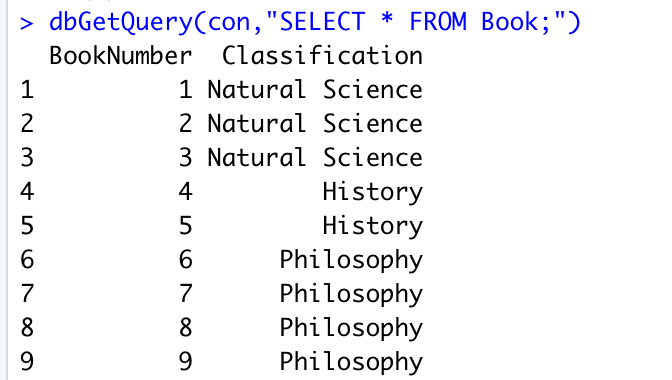
\includegraphics[width=0.4\textwidth]{figures/Q2.1.png}
    \caption{'Book' Tbale}
\end{figure}
(b) 
\begin{figure}[H]
    \centering
    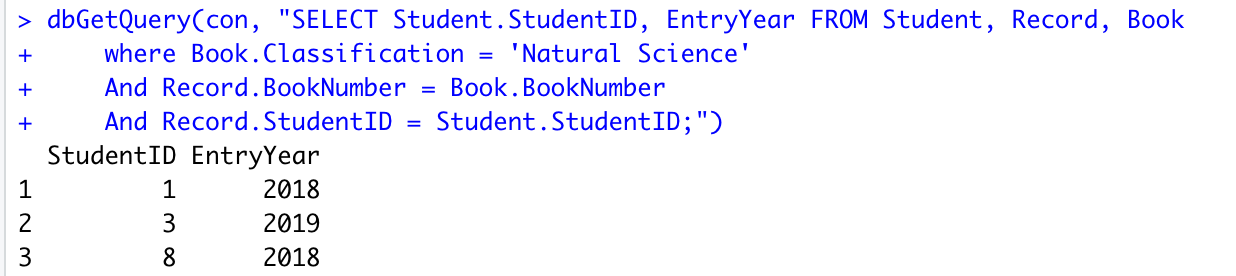
\includegraphics[width=0.7\textwidth]{figures/Q2.2.png}
    \caption{Students who borrowed natural science books}
\end{figure}
(c)
\begin{figure}[H]
    \centering
    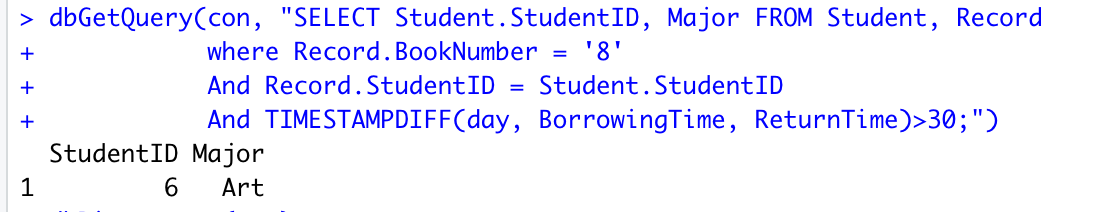
\includegraphics[width=0.7\textwidth]{figures/Q2.3.png}
    \caption{Students who borrowed book 8 for more than 30 days}
\end{figure}

\question{3}{Parse HTML (30\%)}
(a) The result is stored in variable 'comp' in R code.

(b) 


\end{document}